\documentclass[12pt]{article}
\usepackage{graphicx} % Required for inserting images
\usepackage{amsmath, amssymb, amsthm}
\usepackage{inconsolata} 
\usepackage{float}

% Code highlighting (needs --shell-escape in Overleaf if using minted)
\usepackage{listings}
\usepackage{xcolor}

\definecolor{backcolour}{rgb}{0.97,0.97,0.97}
\definecolor{codegreen}{rgb}{0,0.5,0}
\definecolor{codegray}{rgb}{0.4,0.4,0.4}
\definecolor{codepurple}{rgb}{0.58,0,0.82}
\definecolor{keywordblue}{rgb}{0,0,0.8}

\lstdefinestyle{mystyle}{
    basicstyle=\ttfamily\small,
    basicstyle=\fontfamily{zi4}\selectfont\small,
    backgroundcolor=\color{backcolour},   
    commentstyle=\color{codegreen},
    keywordstyle=\color{magenta},
    numberstyle=\tiny\color{codegray},
    stringstyle=\color{codepurple},
    basicstyle=\ttfamily\footnotesize,
    breakatwhitespace=false,         
    breaklines=true,                 
    captionpos=b,                    
    keepspaces=true,                 
    numbers=left,                    
    numbersep=5pt,                  
    showspaces=false,                
    showstringspaces=false,
    showtabs=false,                  
    tabsize=2,
    frame=single,              % adds a frame
    frameround=tttt,           % rounded corners
    rulecolor=\color{gray},    % frame color
    xleftmargin=5pt,
    xrightmargin=5pt
}

\lstset{
    style=mystyle,
    keywordstyle=\color{blue}\bfseries,  % keywords in bold blue
    morekeywords={std::vector, size_t},  % highlight C++ specific stuff
}

% Theorem/definition environments
\newtheorem{definition}{Definition}[section]
\newtheorem{theorem}{Theorem}[section]
\newtheorem{example}{Example}[section]

\title{A CS Guide to Linear Algebra from Scratch}
\author{Strings}
\date{September 2025}

\begin{document}

\maketitle

\begin{abstract}
    This guide was made to help programmers learn linear algebra concepts with a CS perspective with as little background knowledge as possible. The main focus will be on understanding the underlying principles behind practical applications as well as how they interact with the theoretical ones.
\end{abstract}

\section{Introduction}
    Linear algebra is a section of math dedicated to solving systems of linear equations and understanding geometric concepts such as planes and lines. The underlying foundation of linear algebra is vectors and matrices (the plural of "matrix"). From a CS perspective the use of a linear algebra can often be seen in graphics, machine learning and cryptography.
    This paper will be used to build from the basic fundamentals to an above surface knowledge of the topic from the math and its computational implementation.

\section{Basic Concepts}
    \subsection{Scalar}
        A scalar refers to a normal number used in a vector operation.
        They are typically \textbf{real numbers ($\mathbb{R}$)} or \textbf{complex numbers ($\mathbb{C}$)} 
        
    \subsection{Vectors}
        Vectors are one of the biggest building blocks for linear algebra. 
        At its core, a vector is just a list of numbers. For example, consider the vector:

        \begin{equation}
            \mathbf{v} = \begin{bmatrix} 2 \\ 5 \\ -1 \end{bmatrix}
        \end{equation} \\

        This vector has 3 components: 2, 5, -1. \\
        Vectors are used to store information, a common use of a vector is store location.

        \subsubsection{Vector Sets}
            Before we continue lets explain what a \textbf{vector set} is.
            A \textbf{vector set} is a collection of vectors, a bundle of vectors put in set. You think of them as "the vectors we're allowed to consider"
            \textbf{Example:} 
            \begin{equation}
                S = \left\{ 
                    \begin{bmatrix}1\\0\end{bmatrix}, 
                    \begin{bmatrix}0\\1\end{bmatrix}, 
                    \begin{bmatrix}1\\1\end{bmatrix} 
                    \right\}
            \end{equation}
            \\
            Here, the set $S$ contains three vectors in 2D space. Anything not in $S$ is not considered part of this particular set. 
            \\\\
            Later, we'll see a \textbf{vector space}, which is a special type of vector set. In a vector space, you can combine vectors or stretch them, and you’ll never leave the set — everything still stays inside the set.

        \subsubsection{Vector Space}
            Now that we understand what a \textbf{vector set} is — a collection of vectors let's talk about a \textbf{vector space} It is a special type of vector set where you can do two things freely:

            \begin{enumerate}
                \item \textbf{Add any two vectors} from the set, and the result is still in the set.
                \item \textbf{Multiply any vector by a number} (scalar), and the result is still in the set.
            \end{enumerate}

            In other words, a vector space is a “magic basket” of vectors:  
                - You can combine vectors or stretch/shrink them.  
                - No matter what you do, you never leave the basket.

            \textbf{Example:} All 2D vectors form a vector space:
            \begin{equation}
                \mathbb{R}^2 = \left\{ \begin{bmatrix}x \\ y\end{bmatrix} \,\bigg|\, x, y \in \mathbb{R} \right\}
            \end{equation} \\

            In non-klingon this means: A 2D vector contains \textbf{x} and \textbf{y}. \\
            As well, as \textbf{x} and \textbf{y} are \textbf{real numbers}.

            \begin{itemize}
                \item Add two vectors: \\
                \begin{equation}
                    \begin{bmatrix}1 \\ 2 \end{bmatrix} + \begin{bmatrix}3 \\ 4 \end{bmatrix} =         \begin{bmatrix}4 \\ 6 \end{bmatrix} \in \mathbb{R}^2
                \end{equation}
                
                \item Multiply a vector by a scalar: \\
                \begin{equation}
                    2 \cdot \begin{bmatrix}1 \\ 2 \end{bmatrix} =      \begin{bmatrix}2 \\ 4 \end{bmatrix} \in \mathbb{R}^2
                \end{equation}
            \end{itemize}

            Notice how the results stay inside the set — that’s the defining feature of a vector space.
            
        \subsubsection{Algebraic}
            There are multiple ways to view a vector in linear algebra, first is algebraically. Algebraically a vector is a element inside a \textbf{vector space}. \\
            For example, all 3D vectors form $\mathbb{R}^3$

            \begin{itemize}
                \item  You can add component-wise: \\
                \begin{equation}
                  \begin{bmatrix}1 \\ 2 \\ 3 \end{bmatrix} + \begin{bmatrix}4 \\ 5 \\ 6 \end{bmatrix} = \begin{bmatrix}5 \\ 7 \\ 9 \end{bmatrix}
                \end{equation}

                \item  And you can multiply by a scalar: \\
                \begin{equation}
                   2 \cdot \begin{bmatrix}3 \\ -1 \end{bmatrix} = \begin{bmatrix}6 \\ -2 \end{bmatrix}
                \end{equation}
            \end{itemize}
            
        \subsubsection{Geometric}
            \begin{figure}[h]
                \centering
                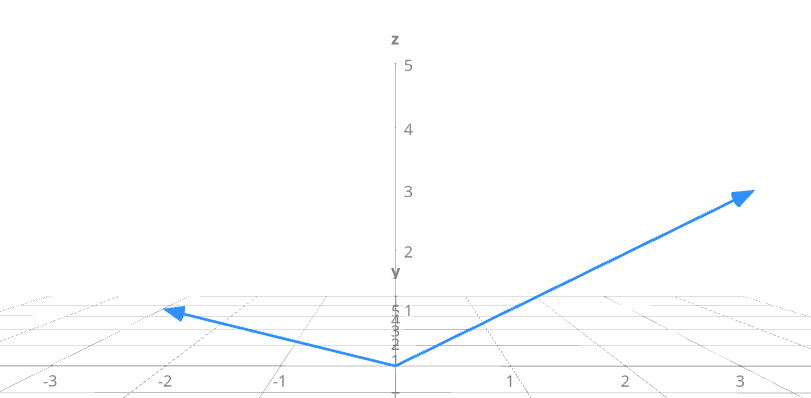
\includegraphics[width=1\textwidth]{1-1.png} 
                \caption{Geometric representation of 2D Vector.}
                \label{fig:1}
            \end{figure}
        
            In a 2D Vector, you can visualize a vector as an \textbf{arrow} pointing from the origin of \textbf{(0, 0)} to a point ($x, y$). \\
            Example:
            \begin{equation}
                \mathbf{v}_1 = \begin{bmatrix} 3 \\ 3 \end{bmatrix}
                \mathbf{v}_2 = \begin{bmatrix} -2 \\ 1 \end{bmatrix}
            \end{equation}
            
            \begin{figure}[H]
                \centering
                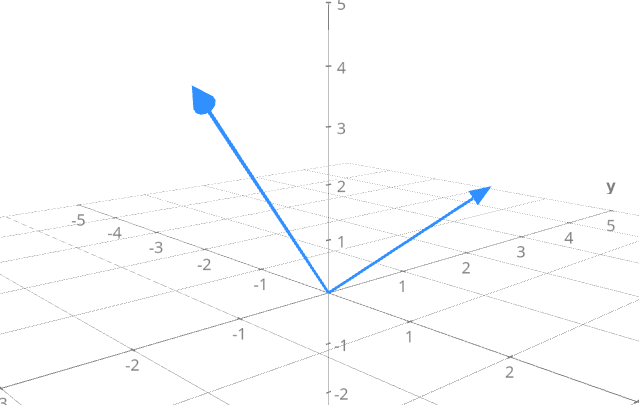
\includegraphics[width=1\textwidth]{1-2.png} 
                \caption{Geometric representation of 3D Vector.}
                \label{fig:2}
            \end{figure}
            
            The same principle works with a 3D vector but pointing to ($x, y, z$) \\
            Example:
            \begin{equation}
                \mathbf{v}_1 = \begin{bmatrix} 1 \\ 1 \\ 2 \end{bmatrix}
                \mathbf{v}_2 = \begin{bmatrix} 1 \\ -2 \\ 4 \end{bmatrix}
            \end{equation}

        \subsubsection{Computer Science Usage}
            In Computer Science common usages of vectors can be:
            \begin{itemize}
                \item A list/array
                \item Method to represent states (e.g., pixel colors, probability, features in ML)
                \item A direction in computer graphics/physics
                \item A velocity or force
                \item Rotation
            \end{itemize}

            \begin{example}[C++ Representation] 
            Here is a example script
            \begin{lstlisting}[language=C++]
#include <iostream>
#include <vector>

int main() {
    std::vector<int> v1 = {3, 4};
    std::vector<int> v2 = {-2, 1};

    std::vector<int> sum(2);
    for (size_t i = 0; i < 2; ++i) {
        sum[i] = v1[i] + v2[i];
    }

    std::cout << "v1 + v2 = [";
    for (size_t i = 0; i < 2; ++i) {
        std::cout << sum[i];
        f (i < 1) std::cout << ", ";
    }
    std::cout << "]" << std::endl;
    return 0;
}
            \end{lstlisting}
            \end{example}

        \subsubsection{Magnitude}
            The magnitude is a property of a vector that can be written with $"\|"$ surrounding a vector, it measures the length (or norm) of a vector from the Pythagorean theorem:
            \begin{equation}
                ||\mathbf{v}|| = \sqrt{v^2_1 + v^2_2 \cdot\cdot\cdot + v^2_n}
            \end{equation}

            Example:
            \begin{equation}
                ||\begin{bmatrix} 3 \\ 4 \end{bmatrix}|| = \sqrt{3^2 + 4^2} = 5
            \end{equation}

            \textbf{Note}: The subscript \textbf{'n'} is the total amount of \textbf{components} in a column when discussing vectors.

    \subsection{Vector Operations}
        \subsubsection{Vector Addition}
            If both vectors are the same size of \textbf{'n'}, you can combine 2 vectors by adding there \textbf{components}.
            \begin{equation}
                \mathbf{a + b} =
                    \begin{bmatrix} a_1 \\ a_2 \\ \cdot \\ \cdot \\ \cdot \\ a_n \end{bmatrix} +
                    \begin{bmatrix} b_1 \\ b_2 \\ \cdot \\ \cdot \\ \cdot \\ b_n \end{bmatrix} =
                    \begin{bmatrix} a_1 + b_2 \\ a_2 + b_2 \\ \cdot \\ \cdot \\ \cdot \\ a_n + a_b \end{bmatrix}
            \end{equation}

            Example:
            \begin{equation}
                \mathbf{a + b} =
                    \begin{bmatrix} 1 \\ 2 \\ 3 \\ 4 \end{bmatrix} +
                    \begin{bmatrix} 5 \\ 6 \\ 7 \\ 8 \end{bmatrix} =
                    \begin{bmatrix} 6 \\ 8 \\ 10 \\ 12 \end{bmatrix}
            \end{equation}

        \subsection{Vector Subtraction}
            If both vectors are the same size of \textbf{'n'}, you can subtract 2 vectors by adding there \textbf{components}.
            \begin{equation}
                \mathbf{a - b} =
                    \begin{bmatrix} a_1 \\ a_2 \\ \cdot \\ \cdot \\ \cdot \\ a_n \end{bmatrix} -
                    \begin{bmatrix} b_1 \\ b_2 \\ \cdot \\ \cdot \\ \cdot \\ b_n \end{bmatrix} =
                    \begin{bmatrix} a_1 - b_2 \\ a_2 - b_2 \\ \cdot \\ \cdot \\ \cdot \\ a_n - a_b \end{bmatrix}
            \end{equation}

            Example:
            \begin{equation}
                \mathbf{a + b} =
                    \begin{bmatrix} 5 \\ 6 \\ 7 \\ 8 \end{bmatrix} -
                    \begin{bmatrix} 1 \\ 2 \\ 3 \\ 4 \end{bmatrix} =
                    \begin{bmatrix} 4 \\ 4 \\ 4 \\ 4 \end{bmatrix}
            \end{equation}

        \newpage
        \subsection{Vector Scalar Multiplication}
            Vector Scalar Multiplication is the act of multiplying a vector by a Scalar. You multiply the scalar to all \textbf{components} inside the vector.

            \begin{equation}
                \mathbb{C} \cdot \mathbf{a} = \mathbb{C} \cdot
                    \begin{bmatrix} a_1 \\ a_2 \\ \cdot \\ \cdot \\ \cdot \\ a_n \end{bmatrix} =
                    \begin{bmatrix}  \mathbb{C} \cdot a_1 \\  \mathbb{C} \cdot a_2 \\ \cdot \\ \cdot \\ \cdot \\  \mathbb{C} \cdot a_n \end{bmatrix}
            \end{equation}

            Example:
            \begin{equation}
                5 \cdot \begin{bmatrix} 1 \\ 2 \\ 3 \\ 4 \end{bmatrix} =
                \begin{bmatrix} 5 \\ 10 \\ 15 \\ 20 \end{bmatrix}
            \end{equation}

        \subsection{}
\end{document}
